\chapter[Transition Rates]{Dimensional Dependence of Optical Transition Rates}
\label{RM}

In this chapter, we focuses on the dimensional dependence of the optical
transition process, such as absorption, spontaneous emission and stimulated
emission behavior in semiconductor when interacting with light. Through
time-dependent perturbation theory and Fermi's Golden Rule, we find out the two
bands optical transition rates, then based on the light interaction
Hamiltonian, time average Poynting vector and matrix element, derive the
absorption coefficient, spontaneous and stimulated emission rates for bulk
semiconductor (3-dimension), quantum well (2-dimension) and nanowire
(1-dimension) structure.

\section{Optical Transition in Semiconductor} \label{OpticalProcess}

All semiconductor optical or photonic devices can be divided into three
groups~\cite{sze2006physics}: (1) devices as light sources that convert
electrical energy into optical radiation (such as LED and Lasers); (2) devices
that detect optical signals (such as photodetectors); (3) devices that convert
optical radiation into electrical energy (such as photovoltaic devices or solar
cells). In addition, all these three groups of photonic devices involve the
generation and recombination of electron-hole pairs.

In order to generate an electron-hole pair, the photon energy has to be greater
than the semiconductor material energy bandgap, $h\gamma\geq{E_g}$, where
$\gamma$ is the frequency of the photon. A variety of material systems have
been employed for different wavelength detection and luminescence due to their
proper bandgap values as depicted in Fig.~\ref{BandgapEmission}. Generally,
GaAs material is used for fiber optical communication applications in the
infrared portion of the electromagnetic spectrum. For visible and near visible
luminescence, where human eyes have higher sensitivity, GaP and CdS materials
are commonly used. GaN and ZnS materials with larger bandgap are primarily used
for violet and ultraviolet applications.

\begin{figure}
  \caption[Schematic representation of various semiconductor materials' energy bandgaps (or wavelengths) with corresponding human eye response.]{Schematic representation of various semiconductor materials' energy bandgaps (or wavelengths) with corresponding human eye response. Adapted from reference~\cite{singh2007semiconductor}}
  \centering
  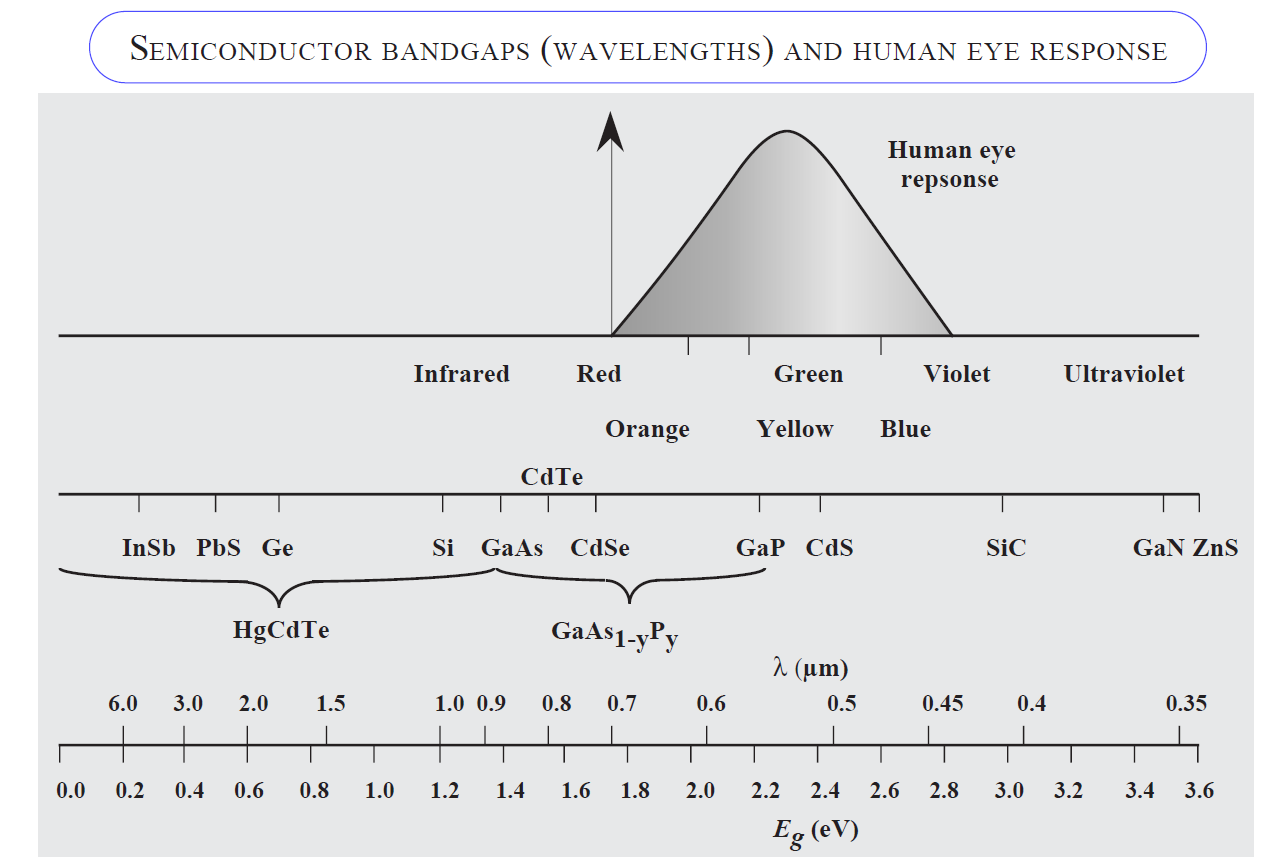
\includegraphics[width=\textwidth]{pictures/RM/BandgapEmission}
  \label{BandgapEmission}
\end{figure}

Besides the energy conservation which requires photon energy to be greater than
the material bandgap, another important condition that is necessary for the
interaction of electron and holes by the perturbation of photon energy.
Figure~\ref{DirectTransition} shows the corresponding energy-momentum (E-k)
plots for two different kinds of bandgap. As indicated in the left part of
Fig.~\ref{DirectTransition}, the conduction band has only one minima, on the
right-hand side, there are two minima. The one with an arrow is the direct
minimum, and the another one is the indirect minimum. Electrons in the direct
minimum of the conduction band and holes at the top of the valence band have
equal momentum; while electrons in the indirect minimum have different
momentum. For direct-bandgap semiconductors, such as GaAs and InAs, the
momentum is conserved and band-to-band transitions may occur with high
probability. The photon energy is then approximately equal to the bandgap
energy of the semiconductor. The radiative transition mechanism is predominant
in direct-bandgap materials. However, for Si and GaP that are indirect bandgap
semiconductors, the probability for interband transitions is extremely small,
since phonons or other scattering agents must participate in the process in
order to conserve momentum~\cite{sze2006physics}.

\begin{figure}
  \caption[Schematic respresentation of optical absorption process in semiconductor (left) direct and (right) indirect bandgap materials.]{Schematic representation of optical absorption process in semiconductor (left) direct and (right) indirect bandgap materials. Adapted from reference~\cite{singh2007semiconductor}.}
  \centering
  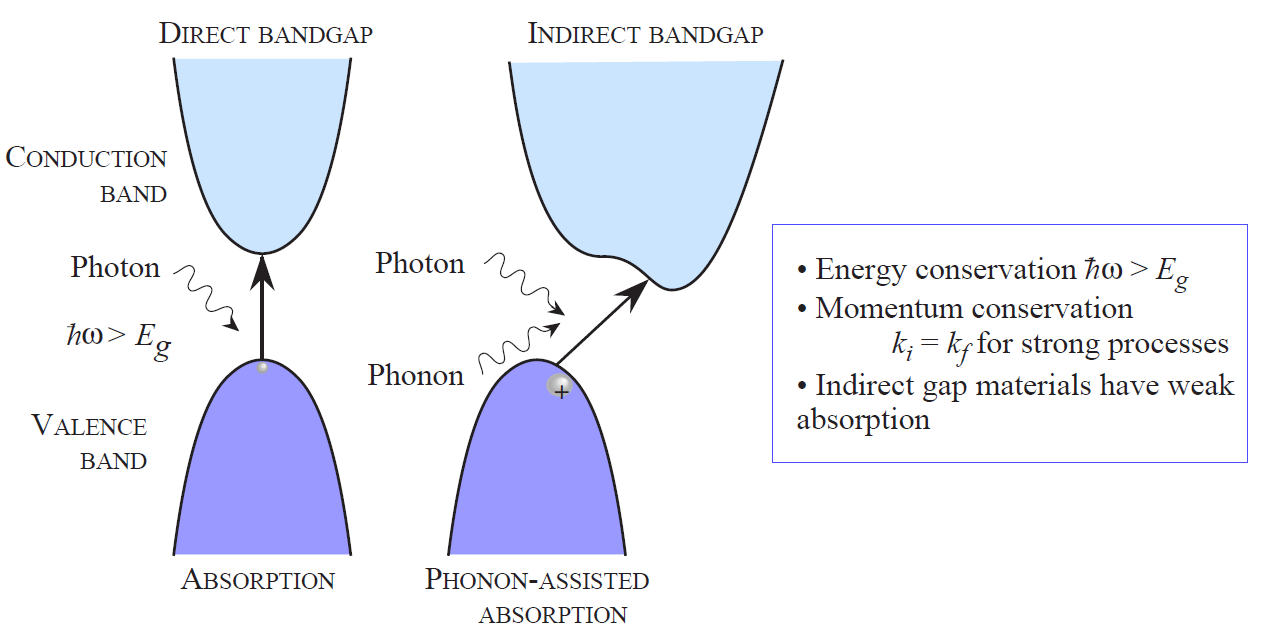
\includegraphics[width=\textwidth]{pictures/RM/DirectTransition}
  \label{DirectTransition}
\end{figure}

There are three main optical processes for interaction between a photon and an electron in a solid as depicted in Fig.~\ref{OpticalProcess}.
\begin{itemize}
  \item An electron excited from a filled state in the valence band to an empty state in the conduction band may absorb one photon. This is called absorption (the left upward arrow in Fig.~\ref{OpticalProcess}) and it is the main process in a photodetector or solar cell.
  \item An electron in the conduction band can spontaneously return to an empty state in the valence band (recombination), with the emission of a photon.  This is called spontaneous emission (the middle downward arrow in Fig.~\ref{OpticalProcess}), as the reverse process of absorption. And this is the primary process for LEDs.
  \item The incoming photon can stimulate the emission of anohter similar photon by recombination, giving out a net of two photons which are coherent (with same energy). This is called stimulated emission (the right downward arrow in Fig.~\ref{OpticalProcess}), and it is the main process in a laser.
\end{itemize}

\begin{figure}
  \caption{Schematic representation of basic interaction of a two-level system and an optical field.}
  \centering
  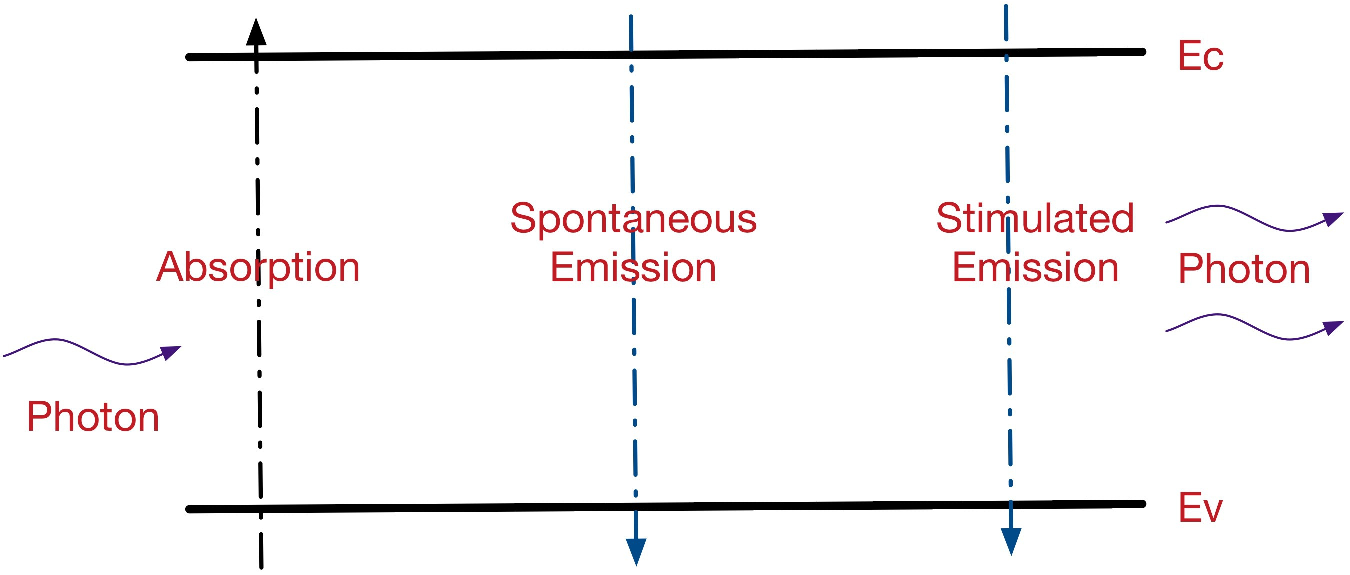
\includegraphics[width=\textwidth]{pictures/RM/OpticalProcess}
  \label{OpticalProcess}
\end{figure}

\section{Optical Transition Rates in Semiconductor} \label{OTR}

In this section, we review the derivation of general optical transition rates
in semiconductor by using time-dependent perturbation theory and Fermi's Golden
Rule.

\subsection{Time-dependent Perturbation Theory} \label{perturbation}

The interaction of light and matter may be analyzed by the time-dependent
perturbation theory (detailed derivation can be found in
Appendix.~\ref{ch:rates}) which gives optical transition rate $W_{if}$ from
initial state 'i' to final state 'f', caused by light as:

\begin{equation}
W_{if}=\frac{2\pi}{\hbar}|H_{fi}^\prime|^2\delta(E_f-E_i-\hbar\omega) + \frac{2\pi}{\hbar}|H_{fi}^\prime|^2\delta(E_f+E_i-\hbar\omega)
\label{eq:OTR}
\end{equation}

Here the prefactor 2 is due to the spins; $H_{fi}^\prime =
\int{{\Phi_f}^\ast(r)H^\prime(r)\Phi_i(r)}d^3r$ is the matrix element defined by
Fermi's Golden Rule~\cite{fermi1950nuclear} that connects the initial state $i$
with the final state $f$ through the perturbation Hamiltonian
${H^\prime}(r,t)=-{\frac{e}{m_0}}\bf{A}(r,t)\cdot~\bf{p}$, where $m_0$ is the
free electron mass, $\bf{A}(r,t)$ is the vector potential accounting for the
presence of the electromagnetic field, and $\bf{p}$ is the momentum operator.
The delta functions indicate the energy conservation, and show the resonance of
photons and electrons for absorption of light (first term) and its emission
(second term).

\subsection{Fermi's Golden Rule} \label{GoldenRule}

When the semiconductor illuminated by light, the interaction between the photons and the electrons in the semiconductor can be described by the Hamiltonian:

\begin{equation}
  \HAM = \frac{1}{2m_0}{(\bm{p}-e\bm{A})}^2+V(\bm{r})
\end{equation}

where $m_0$ is the free electron mass, $e=-|e|$ for electrons, $\bm{A}$ is the vector potential accounting for the presence of the electromagnetic field, and $V(\bm{r})$ is the periodic crystal potential.

The Hamiltonian can be expanded into

\begin{eqnarray}
  & \HAM = \frac{1}{2m_0}{(\bm{p}-e\bm{A})}^2+V(\bm{r})
  &  \approx \HAM_0+\HAM^\prime
\end{eqnarray}

where $\HAM_0$ is the unperturbed Hamiltonian and ${\HAM}^\prime$ is considered as a perturbation due to light

\begin{equation}
\HAM_0=\frac{{\bm{p}}^2}{2m_0}+V(\bm{r})
\end{equation}

\begin{equation}
  \HAM^\prime=-\frac{e}{m_0}\bm{A}\bm{p}
\end{equation}

and consider the coulomb gauge has been used.

\begin{equation}
  \nabla\cdot\bm{A}=0
\end{equation}

noting that $\bm{p}=(\hbar/i)\nabla$, so $\bm{p}\cdot\bm{A}=(\frac{\hbar}{i})\nabla\cdot\bm{A}=\bm{A}\cdot\bm{p}$. And since we know $\bm{p}\approx\hbar{k}\approx\hbar\frac{\pi}{a}$, and $a$ is the lattice constant, usually have a value of $5\mathring{A}$, so $|e\bm{A}|\ll|\bm{p}|$, then we can drop the last term $\frac{e^2{\bm{A}}^2}{2m_0}$, because it is much smaller than the terms linear in $\bm{A}$.

Assume the vector potential for the optical electric field of the form

\begin{eqnarray}
  & \bm{A} = \hat{e}\bm{A}_0\cos{k_{op}\cdot\bm{r}-\omega{t}}
  & = \hat{e}\frac{A_0}{2}e^{ik_{op}\cdot\bm{r}}e^{-i\omega{t}} + \hat{e}\frac{A_0}{2}e^{-ik_{op}\cdot\bm{r}}e^{i\omega{t}}
\end{eqnarray}

where $\bm{k_{op}}$ is the wave vector, $\omega$ is the optical angular frequency, and $\hat{e}$ is a unit vector in the direction of the optical electric field, we have

\begin{equation}
  \bm{E}(\bm{r},t) = -\frac{\partial\bm{A}}{\partial{t}}= -\hat{e}\omega{\bm_{A}}_0\sin{\bm{k_{op}}\cdot\bm{r}-\omega{t}}
\end{equation}

\begin{equation}
  \bm{H}\left( \bm{r,}t \right) = \frac{1}{\mu}\nabla \times \bm{A} = - \frac{1}{\mu}\bm{k_{\bm{\text{op}}}}\bm{\times}\hat{e}A_{0}\sin\left( \bm{k}_{\bm{\text{op}}} \cdot \bm{r} - \omega t \right)
\end{equation}

where we have used the fact that the scalar potential \(\varphi\)
vanishes (\(\rho = 0\)) for the optical field, and \(\mu = \mu_{0}\), the
permeability of the free space. The Poynting vector for the power
intensity \((W/\text{cm}^{2})\) is given by

\begin{equation}
  \bm{P}\left( \bm{r,}t \right) = \bm{E}\left( \bm{r,}t \right) \times \bm{H}\left( \bm{r,}t \right) = \hat{k}\bm{k}_{\bm{\text{op}}}\frac{\omega{A_{0}}^{2}}{\mu}\operatorname{}\left( \bm{k}_{\bm{\text{op}}} \cdot \bm{r} - \omega t \right)
\end{equation}

which is pointing along the direction of wave propagation
\(\bm{k}_{\bm{\text{op}}}\). The time average of the Poynting
flux is simply

\begin{eqnarray}
& \bm{P} = \left| \bm{P}\left( \bm{r,}t \right) \right| = \frac{\omega{A_{0}}^{2}}{2\mu}\bm{k}_{\bm{\text{op}}} \nonumber \\
& = \frac{\omega^{2}{A_{0}}^{2}n_{r}}{2\mu{c}} \nonumber \\
& = \frac{\omega^{2}{A_{0}}^{2}n_{r}\sqrt{\mu_{0}\varepsilon_{0}}}{2\mu_{0}} \nonumber \\
& = \frac{\omega^{2}{A_{0}}^{2}n_{r}\sqrt{\varepsilon_{0}}}{2\sqrt{\mu_{0}}} \nonumber \\
& = \frac{\omega^{2}{A_{0}}^{2}n_{r}\sqrt{\varepsilon_{0}}\sqrt{\varepsilon_{0}}}{2\sqrt{\mu_{0}}\sqrt{\varepsilon_{0}}} \nonumber \\
& = \frac{\omega^{2}{A_{0}}^{2}n_{r}\varepsilon_{0}c}{2}
\end{eqnarray}

Noting the time average of the \(\sin^{2}()\) function is
\(\frac{1}{2}\) and
\(\bm{k}_{\bm{\text{op}}}\bm{=}\omega\sqrt{\mu\varepsilon_{0}} = \frac{\omega}{\nu} = \frac{\omega}{\frac{c}{n_{r}}}\),
\(c = \frac{1}{\sqrt{\mu_{0}\varepsilon_{0}}}\)

The interaction Hamiltonian

\begin{eqnarray}
  & \HAM^{\bm{'}}\left( \bm{r,}t \right)\bm{=} - \frac{e}{m_{0}}\bm{\ A(r,}t\bm{) \cdot p} \nonumber \\
  & \bm{=}\HAM^{\bm{'}}\left( \bm{r} \right)\bm{e}^{\bm{- i\omega t}}\bm{+}\HAM^{\bm{' +}}\left( \bm{r} \right)\bm{e}^{\bm{+ i\omega t}}
\end{eqnarray}

where

\begin{equation}
\HAM^{\bm{'}}\left( \bm{r} \right)\bm{=} - \frac{eA_{0}\bm{e}^{\bm{i}\bm{k}_{\bm{\text{op}}}\bm{\cdot r}}}{2m_{0}}\bm{\  \cdot}\hat{e}\bm{\cdot p}
\end{equation}

The superscript ``+'' means the Hermitian adjoint operator.

The transition rate for the absorption of a photon:

If the electron is at state a initially. And assume \(E_{b} > E_{a}\)

\begin{equation}
W_{\text{abs}} = \frac{2\pi}{\hbar}\left| \left\langle b \middle| \HAM^{\bm{'}}\left( \bm{r} \right) \middle| a \right\rangle \right|^{2}\delta(E_{b} - E_{a} - \hbar\omega)
\end{equation}

The total upward transition rate per unit volume
\((s^{- 1}\text{cm}^{- 3})\) in the crystal taking into account the
probability that state a is occupied and state b is empty:

\begin{equation}
R_{a \rightarrow b} = \frac{2}{V}\sum_{\bm{k}_{a}}^{}{\sum_{\bm{k}_{b}}^{}\frac{2\pi}{\hbar}}\left| {\HAM^{'}}_{\text{ba}} \right|^{2}\delta(E_{b} - E_{a} - \hbar\omega)f_{a}(1 - f_{b})
\end{equation}

where we sum over the initial and final states and assume that the
Fermi-Dirac distribution \(f_{a}\) is the probability that the state a
is occupied. A similar expression holds for \(f_{b}\) with \(E_{a}\)
replaced by \(E_{b}\), and \(\left( 1 - f_{b} \right)\) is the
probability that the state b is empty. The prefactor 2 takes into
account the sum over spins, and the matrix element
\({\HAM^{'}}_{\text{ba}}\) is given by \textbf{Fermi's Golden Rule}

\begin{equation}
{\HAM^{'}}_{\text{ba}} \equiv \left| \left\langle b \middle| \HAM^{\bm{'}}\left( \bm{r} \right) \middle| a \right\rangle \right| = \int_{}^{}{\Psi_{b}^{*}\left( \bm{r} \right)H^{'}\left( \bm{r},t \right)\Psi_{a}\left( \bm{r} \right)d^{3}\bm{r}}
\end{equation}

\subsection{Upward and Downward Transition Rates} \label{UpDownTR}

Similarly, the transition rate for the emission of a photon if an
electron is initially at state b is

\begin{equation}
W_{\text{ems}} = \frac{2\pi}{\hbar}\left| \left\langle a \middle| \HAM^{\bm{'}}\left( \bm{r} \right) \middle| b \right\rangle \right|^{2}\delta(E_{a} - E_{b} + \hbar\omega)
\end{equation}

The downward transition rate per unit volume
\((s^{- 1}\text{cm}^{- 3})\) is

\begin{equation}
R_{b \rightarrow a} = \frac{2}{V}\sum_{\bm{k}_{a}}^{}{\sum_{\bm{k}_{b}}^{}\frac{2\pi}{\hbar}}\left| {\HAM^{' +}}_{\text{ab}} \right|^{2}\delta(E_{a} - E_{b} + \hbar\omega)f_{b}(1 - f_{a})
\end{equation}

Using the even property of the delta function,
\(\delta\left( - x \right) = \delta\left( x \right)\), and
\({\HAM^{'}}_{\text{ba}} = {\HAM^{' +}}_{\text{ab}}\), the net upward
transition rate per unit volume can be written as

\begin{equation}
R = R_{a \rightarrow b} - R_{b \rightarrow a} = \frac{2}{V}\sum_{\bm{k}_{a}}^{}{\sum_{\bm{k}_{b}}^{}\frac{2\pi}{\hbar}}\left| {\HAM^{'}}_{\text{ba}} \right|^{2}\delta(E_{b} - E_{a} - \hbar\omega)(f_{a} - f_{b})
\end{equation}

The absorption coefficient \(\alpha(1/cm)\) in the crystal is the
fraction of photons absorbed per unit distance:

\begin{equation}
\alpha = \frac{\text{Number\ of\ photons\ absorbed\ per\ second\ per\ unit\ volume}}{\text{Number\ of\ injected\ photons\ per\ second\ per\ unit\ area}}
\end{equation}

The injected number of photons per second per unit area is the optical
intensity \(P(W/\text{cm}^{2})\) divided by the energy of a photon
\(\hbar\omega\):

\begin{equation}
\alpha\left( \hbar\omega \right) = \frac{R}{\frac{P}{\hbar\omega}} = \frac{\hbar\omega}{(\frac{n_{r}c\epsilon_{0}\omega^{2}A_{0}^{2}}{2})}R
\end{equation}

Using the long wavelength approximation that
\(\bm{A}\left( \bm{r} \right) = \bm{A}e^{i\bm{k}_{\bm{\text{op}}}\bm{\cdot}r}\bm{\approx A}\),
we find that the matrix element can be written in terms of the momentum
matrix element

\begin{equation}
{\HAM^{'}}_{\text{ba}} = - \frac{e}{m_{0}}\bm{\ A \cdot}\left\langle b \middle| \bm{p} \middle| a \right\rangle\bm{=}\frac{eA_{0}}{2m_{0}}\bm{\  \cdot}\hat{e}\bm{\cdot}\bm{p}_{\text{ba}}
\end{equation}

The absorption coefficient becomes

\begin{eqnarray}
  & \alpha\left( \hbar\omega \right) = C_{0}\frac{2}{V}\sum_{\bm{k}_{a}}^{}{\sum_{\bm{k}_{b}}^{}\left| \hat{e}\bm{\cdot}\bm{p}_{\text{ba}} \right|^{2}}\delta(E_{b} - E_{a} - \hbar\omega)(f_{a} - f_{b}) \nonumber \\
  & C_{0} = \frac{\pi e^{2}}{n_{r}\varepsilon_{0}cm_{0}^{2}\omega}
\end{eqnarray}

We can see that the factors containing ${A_0}^2$ are canceled because the
linear optical absorption coefficient is independent of the optical intensity.

\subsection{Photonic Modes Density}\label{photonic-density-of-states}

In order to find the density of states for the photon field, We need to
first calculate the number of modes in a cube (mode density) of
refractive index \(\mathbf{n}_{\mathbf{r}}\) and side length \emph{\textbf{L}}
in a frequency interval between \(\nu\) and \(\nu + d\nu\), assuming
that \emph{\textbf{L}} is much larger than the wavelength of the mode
under consideration. As is usual, the photon field can be describes by a
plane wave:

\begin{equation}
  e^{i\bm{k}\cdot\bm{r}} = e^{ik_{x}x + ik_{y}y + ik_{z}z}
\end{equation}

Using the periodic boundary conditions that the wave function should be
periodic in the x, y and z directions with a period L.

\begin{equation}
  k_{x} = l\frac{2\pi}{L}\ ,\ k_{y} = m\frac{2\pi}{L}\text{\ and}\ k_{z} = n\frac{2\pi}{L}
\end{equation}

With

\begin{equation}
k^{2} = k_{x}^{2} + k_{y}^{2} + k_{z}^{2} = {(\frac{2\pi}{L})}^{2} = {(\frac{2\pi\nu n_{r}}{c})}^{2}
\end{equation}

A combination of l, m and n describes a mode. The volume of a state in
the k-space is \(\left( \frac{2\pi}{L} \right)^{3}\). Therefore the
number of modes per unit volume of k-space in the frequency range 0 to
\(\nu\) (or having wavevectors in the interval 0 to \emph{k}) is
obtained by dividing the volume of a sphere with radius \(\nu\) (or
\emph{k}) by the volume per mode\(\left( \frac{2\pi}{L} \right)^{3}\).

\begin{eqnarray}
   & N_{v} = \frac{{8\pi^{3}v}^{3}n_{r}^{3}L^{3}}{3c^{3}\pi^{2}}
   & = \frac{k^{3}L^{3}}{3\pi^{2}}
\end{eqnarray}

The enclosed volume is \(V_{v} = L^{3}\), the number of modes per unit
volume in the frequency range 0 to \(\nu\) is

\begin{equation}
  \frac{N_{v}}{V_{v}} = \frac{{8\pi v}^{3}n_{r}^{3}}{3c^{3}}\ \ \ \ \ \ \ \ (\text{cm}^{- 3})
  \label{eq:numberofmodes}
\end{equation}

As the initial assumption that the enclosure size \emph{\textbf{L}} is much
larger than the wavelength of the enclosed mode. This implies a large mode
density closely spaced in frequency; however, as a nanowire, the diameter and
length of the lasing cavity comes to subwavelength, we may have to alter the
mode density function. Taking the derivative of Eq.~\ref{eq:numberofmodes} with
respect to \(\nu\) gives us the mode density per unit frequency interval per
unit volume between \(\nu\) and \(\nu + d\nu\),

\begin{equation}
n_{v} = \frac{1}{V_{v}}\frac{\text{dN}_{v}}{\text{dv}} = \frac{{8\pi v}^{2}n_{r}^{2}}{c^{3}}\ \ \ \ \ \ \ \ (\text{s.cm}^{- 3})
\end{equation}

Similarly, the mode density per unit energy interval is

\begin{equation}
n_{\varepsilon} = \frac{8\pi{n_{r}}^{3}\varepsilon^{2}}{\left( 2\pi \right)^{3}h^{3}c^{3}} = \frac{{n_{r}}^{3}\varepsilon^{2}}{\pi^{2}\hbar^{3}c^{3}}\quad
\text{cm}^{- 3}{(eV)}^{- 1}
\end{equation}

This equation gives the number of electromagnetic modes with different
l, m, n, per unit volume, having energy in the interval between
\(\varepsilon\text{\ and}\ {\varepsilon +}\mathbf{d}\varepsilon\).

The radiation density of the modes in a frequency interval \(\text{dv}\)
is given by

\begin{equation}
  \varphi\left( v \right)d\nu = vn_{v}u_{v}\text{dv}
\end{equation}

And in an energy interval \(\mathbf{d}\varepsilon\) by

\begin{equation}
\varphi\left( \mathcal{E} \right)d\mathcal{E} = hvn_{\varepsilon}u_{\varepsilon}d\varepsilon
\end{equation}

\(\text{hv}\) on the right-hand side is the energy per photon, the second term
\(n_{\varepsilon}\) is the mode density, and the third term \(u_{\varepsilon}\)
is the average number of photons per mode in the energy interval between
\(\varepsilon\text{\ and}\ {\varepsilon +}\mathbf{d}\varepsilon\), which is the
same as the occupation factor that following the Bose-Einstein statistics for photons:

\begin{equation}
  u_{\varepsilon} = \frac{1}{e^{\frac{\hbar\omega_{k}}{k_{B}T}} - 1}
  \label{eq:occupationfactor}
\end{equation}

Then the photon density per unit energy interval can be defined as $N_{p} =
n_{\varepsilon}u_{\varepsilon}$:

\begin{equation}
  N_{p} = \frac{{n_{r}}^{3}\varepsilon^{2}}{\pi^{2}\hbar^{3}c^{3}}\frac{1}{e^{\frac{\varepsilon}{k_{B}T}} - 1} \quad \text{cm}^{- 3}{(eV)}^{- 1}
  \label{eq:photondensity}
\end{equation}

\section{The Einstein Relations}\label{einstein-relations}

Consider two energy levels \(\mathbf{\varepsilon}_{1}\) and
\(\mathbf{\varepsilon}_{2}\) with populations \(\mathbf{N}_{1}\) and
\(\mathbf{N}_{2}\) in an atomic system in thermal equilibrium.
\(\mathbf{\varepsilon}_{2}\) is larger than \(\mathbf{\varepsilon}_{1}\) and
normally \(\mathbf{N}_{2}\) is smaller than \(\mathbf{N}_{1}\). In such a
system, the rate of the upward transition must equal the rate of the downward
transitions.

Then define Einstein's \(B_{12}\) Coefficients as

\begin{equation}
  B_{12} = \frac{2\pi}{\hbar}\left| {\HAM^{'}}_{12} \right|^{2}
\end{equation}

where \(B_{12}\) is known as the Einstein coefficient for stimulated
upward transitions, or absorption rate per incident photon within an
energy interval, (eV/s). So the upward transition rate per unit volume
(\(s^{- 1}\text{cm}^{- 3}\)) is proportional to \(\mathbf{N}_{1}\) and
the radiation density \(\varphi\left( v \right)\),

\begin{equation}
  r_{12}{= B}_{12}\mathbf{N}_{1}\varphi\left( v \right)
\end{equation}

Thus, for the total upward transition rate per unit volume
(\(s^{- 1}\text{cm}^{- 3}\)) for a broad spectrum is

\begin{equation}
  R_{12}{= B}_{12}S(E_{21})
\end{equation}

where

\begin{equation}
  S\left( E_{21} \right) = N\left( E_{21} \right)n_{\varepsilon}
\end{equation}

is the number of photons per unit volume per energy interval with a
dimension of \(\text{cm}^{- 3}{(eV)}^{- 1}\),

\begin{equation}
  n_{\varepsilon} = \frac{1}{e^{\frac{E_{21}}{k_{B}T}} - 1}
\end{equation}
is the number of photons per state at an optical energy \(E_{21} \).

If we take into account the occupation probabilities of level 1 and
level 2 using Fermi-Dirac distributions, \(f_{1}\) and \(f_{2}\),
respectively, the expression for \(R_{12}\) will be modified,

\begin{eqnarray}
   & R_{12}{( = r}_{12}(E_{21})dE) = \frac{1}{V}\sum_{k}^{}{B_{12}\delta\left( E_{2} - E_{1} - \hbar\omega_{k} \right)}2n_{\varepsilon}\mathbf{\cdot}f_{1}(1 - f_{2})\nonumber \\
   & = B_{12}f_{1}(1 - f_{2})S\left( E_{21} \right)
\end{eqnarray}

Where \(r_{12}(E_{21})dE\) means that the upward transition rate per unit
volume has been integrated for a light with a spectral width \(\text{dE}\) near
\({E = E}_{21}\), \(\ r_{12}(E)\) is the number of $1\rightarrow2$ transitions
per second per unit volume per energy interval (\(s^{- 1}\text{cm}^{-
3}\text{eV}^{- 1}\)).

Similarly, a stimulated emission rate per unit volume can be given

\begin{equation}
  R_{21}^{\text{stim}} = r_{21}^{\text{stim}}(E)dE = B_{21}f_{2}(1 - f_{1})S\left( E_{21} \right)
\end{equation}

In the case of spontaneous emission, where the photons created by
recombination escape, the spontaneous emission rate per unit volume is
independent of the photon density and is given by

\begin{equation}
  R_{21}^{\text{spon}} = r_{21}^{\text{spon}}(E)dE = A_{21}f_{2}(1 - f_{1})
\end{equation}

\(A_{21}\) is the Einstein coefficient for spontaneous emission. As A
and B coefficient are not changed whether in thermal equilibrium or not,
we can use the following properties in the future. At thermal
equilibrium, there is only one Fermi level; therefore \(F_{1} = F_{2}\).
We balance the total downward transition rate with the upward transition
rate:

\begin{equation}
{{R_{12} = R}_{21}^{\text{stim}} + R}_{21}^{\text{spon}}
\end{equation}

or

\begin{equation}
B_{12}f_{1}\left( 1 - f_{2} \right)S\left( E_{21} \right) = B_{21}f_{2}\left( 1 - f_{1} \right)S\left( E_{21} \right) + A_{21}f_{2}(1 - f_{1})
\end{equation}

We have

\begin{equation}
\frac{A_{21}}{{B_{12}e}^{\frac{E_{21}}{k_{B}T}} - B_{21}} = N\left( E_{21} \right)\frac{1}{e^{\frac{E_{21}}{k_{B}T}} - 1}
\end{equation}

By comparing the left- and right-hand sides, we find \(B_{12} = B_{21}\), and

\begin{equation}
  \frac{A_{21}}{B_{21}} = N\left( E_{21} \right) = \frac{n_{r}^{3}E_{21}^{2}}{\pi^{2}\hbar^{3}c^{3}}
\end{equation}

Thus, the ratio of the stimulated and spontaneous emission rate is:

\begin{equation}
  \frac{R_{21}^{\text{stim}}}{R_{21}^{\text{spon}}} = \frac{B_{21}f_{2}\left( 1 - f_{1} \right)S\left( E_{21} \right)}{A_{21}f_{2}(1 - f_{1})} = n_{\varepsilon}
  \label{eq:sponstiratio}
\end{equation}
which is the number of photons per state.

\section[Interband Transition Rates]{Dimensional Dependence of Interband Transition Rates}\label{ITR}

Optical interband transition rates are strong function of dimensionality.
Shrinking the size of the devices not only introduced the confinement of
electron and hole movement, but also modified the optical interband transition
rates dramatically. 

\subsection{Interband Transition Rates for a Bulk Semiconductor} \label{3DTR}

Here, we evaluate the optical matrix element:

\begin{equation}
{\HAM^{'}}_{\text{ba}} = \bm{\ }\left\langle b \middle| - \frac{e\bm{A(r)}}{m_{0}}\bm{\cdot p} \middle| a \right\rangle
\end{equation}

The vector potential for the optical field is

\begin{equation}
\bm{A}\left( \bm{r} \right)\bm{= A}{\cdot e}^{i\bm{k}_{\bm{\text{op}}} \cdot r} = \frac{\hat{e}A_{0}}{2}e^{i\bm{k}_{\bm{\text{op}}} \cdot r}
\end{equation}

The Bloch functions for electrons in the valence band \(E_{a}\) and the
conduction band \(E_{b}\) are:

\begin{equation}
\Psi_{a}\left( \bm{r} \right) = u_{v}(\bm{r})\frac{e^{i\bm{k}_{\bm{v}} \cdot r}}{\sqrt{V}}
\end{equation}

\begin{equation}
\Psi_{b}\left( \bm{r} \right) = u_{c}(\bm{r})\frac{e^{i\bm{k}_{\bm{c}} \cdot r}}{\sqrt{V}}
\end{equation}

where \(u_{v}(\bm{r})\) and \(u_{c}(\bm{r})\) are the periodic
parts of the Bloch functions, and the remainders are the envelope
functions (plane waves) for a free electron. The momentum matrix element
is derived from

\begin{eqnarray}
  & {\HAM^{'}}_{\text{ba}} = - \frac{eA_{0}}{2m_{0}}\bm{\ }\hat{e}\bm{\cdot}\int_{}^{}{\Psi_{b}^{*}e^{i\bm{k}_{\bm{\text{op}}}\bm{\cdot}r}\bm{p}\Psi_{a}d^{3}\bm{r}} \nonumber \\
  & = - \frac{eA_{0}}{2m_{0}}\bm{\ }\hat{e}\bm{\cdot}\int_{}^{}{u_{c}(\bm{r})e^{i\bm{k}_{\bm{c}} \cdot r}e^{i\bm{k}_{\bm{\text{op}}}\bm{\cdot}r}\left\lbrack \left( \frac{\hbar}{i}\nabla u_{v}(\bm{r}) \right)e^{i\bm{k}_{\bm{v}} \cdot r} + \hbar\bm{k}_{\bm{v}}u_{v}(\bm{r})e^{i\bm{k}_{\bm{v}} \cdot r} \right\rbrack\frac{d^{3}\bm{r}}{V}} \nonumber \\
  & \approx - \frac{eA_{0}}{2m_{0}}\bm{\ }\hat{e}\bm{\cdot}\int_{\Omega}^{}{{u_{c}}^{*}(\bm{r}){\frac{\hbar}{i}\nabla u}_{v}(\bm{r})}\frac{d^{3}\bm{r}}{\Omega}\int_{V}^{}e^{i{\bm{( -}\bm{k}_{\bm{c}}\bm{+}\bm{k}_{\bm{\text{op}}}\bm{+ k}}_{\bm{v}}) \cdot r}\frac{d^{3}\bm{r}}{V} \nonumber \\
  & = - \frac{eA_{0}}{2m_{0}}\bm{\ }\hat{e}\bm{\cdot}\bm{p}_{\text{cv}}\delta_{{\bm{k}_{\bm{c,}}\bm{k}_{\bm{\text{op}}}\bm{+ k}}_{\bm{v}}}
\end{eqnarray}

\begin{equation}
\bm{p}_{\text{cv}}\bm{=}\int_{\Omega}^{}{{u_{c}}^{*}(\bm{r}){\frac{\hbar}{i}\nabla u}_{v}(\bm{r})}\frac{d^{3}\bm{r}}{\Omega}
\end{equation}

where we noted that
\(\left\lbrack {u_{c}}^{*}(\bm{r})\frac{\hbar}{i}\nabla u_{v}(\bm{r}) \right\rbrack\)
and
\(\left\lbrack {u_{c}}^{*}(\bm{r})u_{v}(\bm{r}) \right\rbrack\)
are periodic functions with the period of a unit cell, whereas the
envelope functions are slowly varying functions over a unit cell.
Therefore, the integral over \(d^{3}\bm{r}\) can be separated into
the product of two integrals, one over the unit cell \(\Omega\) for the
periodic part, and the other over the slowly varying part. In another
word, we use the approximation:

\begin{equation}
\int_{V}^{}\left\lbrack {u_{c}}^{*}\left( \bm{r} \right){\frac{\hbar}{i}\nabla u}_{v}\left( \bm{r} \right) \right\rbrack F(\bm{r})d^{3}\bm{r \approx}\int_{V}^{}{F(\bm{r})}d^{3}\bm{r}\int_{\Omega}^{}{{u_{c}}^{*}(\bm{r}){\frac{\hbar}{i}\nabla u}_{v}(\bm{r})}\frac{d^{3}\bm{r}}{\Omega}
\end{equation}

where \(F(\bm{r})\) is slowly varying over a unit cell, and we have
used the periodic property of the Bloch periodic functions

\begin{equation}
{u_{c}}^{*}\left( \bm{r} \right){\frac{\hbar}{i}\nabla u}_{v}\left( \bm{r} \right) = \sum_{\bm{G}}^{}{\bm{C}_{\bm{G}}e^{i\bm{G} \cdot r}}
\end{equation}

where the vectors \(\bm{G}^{\bm{'}}s\) are the reciprocal
lattice vectors. Because \(F\left( \bm{r} \right)\) is slowly
varying over a unit cell, we may approximate
\(F\left( \bm{r + R} \right) = F\left( \bm{R} \right)\) and put
it outside of the integral over a unit cell. Here the \emph{\textbf{R}}s
are the lattice vectors, and
\(e^{i\bm{G} \cdot \bm{R}} = 1\).\(\omega\) is the volume
of a unit cell. Note that the orthogonal property

\begin{eqnarray}
  & \int_{\Omega}^{}{{u_{c}}^{*}u_{v}d^{3}\bm{r} = 0}, \nonumber \\
  & \frac{1}{\Omega}\int_{\Omega}^{}{{u_{c}}^{*}u_{c}d^{3}\bm{r} = \frac{1}{\Omega}\int_{\Omega}^{}{{u_{v}}^{*}u_{v}d^{3}\bm{r} = 1}}
\end{eqnarray}

From the matrix element, we see the momentum conservation

\begin{equation}
\hbar\bm{k}_{c} = \hbar\bm{k}_{v} + \hbar\bm{k}_{\text{op}}
\end{equation}

is obeyed. The electron at the final state has its crystal momentum
\(\hbar\bm{k}_{\text{c\ }}\)equal to its initial momentum\(\hbar\bm{k}_{v}\)
plus the photon momentum\(\hbar\bm{k}_{\text{op}}\). Because
\(\bm{k}_{\text{op}}\sim\frac{2\pi}{\lambda_{0}}\), and the magnitudes
\(\bm{k}_{\text{c\ }},\bm{k}_{\text{v\ }}\) are of the order\(\
\frac{2\pi}{a_{0}}\), where \(a_{0}\ \)is the lattice constant of the
semiconductors, which is typically of the order $5.5\mathring{A}$  and is much
smaller than we may ignore \(\bm{k}_{\text{op}}\) and obtain

\begin{equation}
{\HAM^{'}}_{\text{ba}} \approx - \frac{eA_{0}}{2m_{0}}\bm{\ }\hat{e}\bm{\cdot}\bm{p}_{\text{cv}}\delta_{{\bm{k}_{\bm{c,}}\bm{k}}_{\bm{v}}}
\end{equation}

which is the \textbf{K}-selection Rule.

\begin{enumerate}
\def\labelenumi{\arabic{enumi})}
\item
  Interband momentum matrix element \(\bm{p}_{\text{cv}}\) depend
  only on the periodic parts of the Bloch functions
  (\(u_{c}\text{\ and\ }u_{v}\)),
\item
  The original optical momentum matrix element
  \(\bm{p}_{\text{ab}}\), depends on the full wave functions (i.e.
  including the envelope function).
\end{enumerate}

Using the \textbf{K}-selection rule in the matrix element, we find that
the absorption coefficient for a bulk semiconductor is

\begin{eqnarray}
& \alpha\left( \hbar\omega \right) = C_{0}\frac{2}{V}\sum_{\bm{k}_{a}}^{}{\sum_{\bm{k}_{b}}^{}\left| \hat{e}\bm{\cdot}\bm{p}_{\text{cv}} \right|^{2}}\delta(E_{c} - E_{v} - \hbar\omega)(f_{v} - f_{c}) \nonumber \\
  & C_{0} = \frac{\pi e^{2}}{n_{r}\varepsilon_{0}cm_{0}^{2}\omega}
\end{eqnarray}

where the Fermi-Dirac distributions for the electrons in the valence
bend and in the conduction band are, respectively.

\begin{equation}
f_{v}\left( k \right) = \frac{1}{1 + e^{\frac{(E_{v}\left( k \right) - F_{v})}{\text{KT}}}}
,
f_{c}\left( k \right) = \frac{1}{1 + e^{\frac{(E_{c}\left( k \right) - F_{c})}{\text{KT}}}}
\end{equation}

Assume:

\begin{enumerate}
\def\labelenumi{\arabic{enumi})}
\item
  \(\bm{k}_{\text{c\ }} = \bm{k}_{\text{v\ }} = \bm{k}\)\textbf{,}
  \(F_{v} = F_{c} = E_{F}\) (thermal equilibrium)
\item
  \(f_{v} = 1\ and\ f_{c} = 0\)
\item
  \(\left| \hat{e}\bm{\cdot}\bm{p}_{\text{cv}} \right|^{2}\)
  is independent of \(\bm{k}\) and denote the absorption spectrum at
  thermal equilibrium.
\end{enumerate}

\begin{equation}
\alpha\left( \hbar\omega \right) = C_{0}\left| \hat{e}\bm{\cdot}\bm{p}_{\text{cv}} \right|^{2}\int_{}^{}\frac{2d^{3}\bm{k}}{\left( 2\pi \right)^{3}}\delta(E_{g} + \frac{\hbar^{2}\bm{k}^{\bm{2}}}{2m_{r}^{*}} - \hbar\omega)
\end{equation}

where used the reduced effective mass \(m_{r}^{*}\)

\begin{eqnarray}
  \begin{aligned}
  & E_{c} = E_{g} + \frac{\hbar^{2}\bm{k}^{\bm{2}}}{2m_{r}^{*}}
  & E_{v} = - \frac{\hbar^{2}\bm{k}^{\bm{2}}}{2m_{r}^{*}} \nonumber \\
  & \frac{1}{m_{r}^{*}} = \frac{1}{m_{e}^{*}} + \frac{1}{m_{h}^{*}}
  \end{aligned}
\end{eqnarray}

Here all energies are measured from the top of the valence band.
Therefore, both \(E_{c}\text{\ and\ }F_{c}\) contain the band-gap energy
\(E_{g}\). Let

\begin{eqnarray}
  & X = E_{g} + E - \hbar\omega
  & E = \frac{\hbar^{2}\bm{k}^{\bm{2}}}{2m_{r}^{\ast}}
\end{eqnarray}

we find, by a change of variables, the integration can be carried out
with the contribution at \(X = 0,\ and\ E = {\hbar\omega - E}_{g}\)

\begin{eqnarray}
  & \alpha_{3D}\left( \hbar\omega \right) = C_{0}\left| \hat{e}\bm{\cdot}\bm{p}_{\text{cv}} \right|^{2}\rho_{r}\left( {\hbar\omega - E}_{g} \right)(f_v-f_c)  \\
  & \rho_{r}\left( {\hbar\omega - E}_{g} \right) = \frac{1}{2\pi^{2}}{(\frac{2m_{r}^{*}}{\hbar^{2}})}^{\frac{3}{2}}\left( {\hbar\omega - E}_{g} \right)^{\frac{1}{2}}
\end{eqnarray}

Therefore, the absorption coefficient depends on the momentum matrix
element and the joint optical density of states. Below the band-gap
energy \(E_{g}\), the absorption does not occur because the photons see
a forbidden band gap.

For the derivation of spontaneous emission rate, we start from the absorption
spectrum within a spectral width \(\text{dE}\):

\begin{eqnarray}
   &  \alpha\left( E_{21} \right)dE = \frac{r_{\text{net}}^{\text{abs}}\left( E_{21} \right)\text{dE}}{P\left( E_{21} \right)\frac{c}{n_{r}}} \nonumber \\
   & = \frac{n_{r}}{c}B_{12}\left( f_{1} - f_{2} \right)
\end{eqnarray}
where \(P\left( E_{21} \right)\) is the irradiance of the photon beam or energy
crossing the unit area in unit time (\(\text{cm}^{- 3}\text{eV}^{- 1}\)).

The ratio of the spontaneous emission spectrum and the absorption
spectrum can be expressed as:

\begin{eqnarray}
  & \frac{r_{21}^{\text{spon}}\left( E_{21} \right)}{\alpha\left( E_{21} \right)} = \frac{A_{21}f_{2}\left( 1 - f_{1} \right)}{\frac{n_{r}}{c}B_{12}\left( f_{1} - f_{2} \right)}
  & = \frac{c}{n_{r}}\cdot{N}\left( E_{21} \right)\frac{1}{e^{\frac{(E_{21} - F)}{k_{B}T}} - 1}
\end{eqnarray}

or

\begin{equation}
  r_{21}^{\text{spon}}\left( E_{21} \right) = (\frac{n_{r}^{2}E_{21}^{2}}{\pi^{2}\hbar^{3}c^{2}})\frac{1}{e^{\frac{{(E}_{21} - F)}{k_{B}T}} - 1}\alpha\left( E_{21} \right)
\end{equation}

and \(F = F_{2} - F_{1}\) is the quasi-Fermi level separation. Now, the
spontaneous emission rate can be carried out as:

\begin{equation}
r_{3D}^{\mathrm{spon}}(\hbar\omega)=\frac{{n_r}{e^2}\omega{p_{cv}}^2}{{\pi}\epsilon_0{m_0}^2C^3{\hbar}}\frac{{{m_r}^\ast}^{3/2}}{2{\pi}^2{\hbar}^3}{\sqrt{(\hbar\omega-E_g)}}f_c(1-f_v)
\end{equation}

In addition, based on the relationship between spontaneous emission and
stimulated emission as in Eq.~\ref{eq:sponstiratio}, the stimulated emission
can also be derived as:

\begin{equation}
       r_{3D}^{\mathrm{sti}}(\hbar\omega)= \left(\frac{n_r\omega{e^2}(1+u_\varepsilon)}{3\pi\hbar{c^3}\epsilon_0m_0^2}\right){|\hat{e}\cdot\bf{p}_{cv}|^2}f_c(1-f_v) \frac{1}{2\pi^2}(\frac{2m_r^\ast}{\hbar^2})^{3/_2}(\hbar\omega-E_g)^{1/_2}
       \label{eq:3Dsti}
\end{equation}

\subsection{Interband Transition Rates in A Quantum
Well}\label{2DTR}

The central cell functions in the quantum wells are relatively
unaffected by the presence of the confining potential. There are only
two changes compared to bulk semiconductor, first, the nature of
wavefunction for the low lying states are confined to the well region,
second, the density of the state have the usual step-like form for
parabolic 2-dimensional bends.

Ignore the excitonic effects due to the Coulomb interaction between
electrons and holes.

Within a two-band model, the Bloch wave functions can be described by

\begin{equation}
\Psi_{a}\left( \bm{r} \right) = u_{v}(\bm{r})\frac{e^{i\bm{k}_{\bm{t}} \cdot \rho}}{\sqrt{A}}g_{m}(z)
\end{equation}

for a hole wave function in the heavy-hole or a light-hole subband m.
and

\begin{equation}
\Psi_{b}\left( \bm{r} \right) = u_{c}(\bm{r})\frac{e^{i\bm{k}_{\bm{t}} \cdot \rho}}{\sqrt{A}}\Phi_{n}(z)
\end{equation}

for an electron in the conduction subband n. The momentum matrix element
\(\bm{p}_{\text{ba}}\) is given by

\begin{equation}
\bm{p}_{\text{ba}}\bm{=}\left\langle \Psi_{b} \middle| \bm{p} \middle| \Psi_{a} \right\rangle \approx \left\langle u_{c} \middle| \bm{p} \middle| u_{v} \right\rangle\delta_{k_{t},k_{t}^{'}}\ I_{\text{hm}}^{\text{en}}
\end{equation}

where

\begin{equation}
I_{\text{hm}}^{\text{en}} = \int_{- \infty}^{+ \infty}{\text{dz}\Phi_{n}^{*}(z)}g_{m}(z)
\end{equation}

\begin{itemize}
\item
  This is the overlap integral of the conduction and valence band
  envelope functions
\item
  \textbf{K}-Selection rule applied
\item
  Take into account the quantization of the electron and hole energies
  \(E_{a}\text{\ and\ }E_{b}\)
\end{itemize}

\begin{equation}
E_{a} = E_{\text{hm}} - \frac{\hbar^{2}\bm{k}_{\bm{t}}^{2}}{2m_{h}^{*}}
\end{equation}

\begin{equation}
E_{b} = {E_{g} + E}_{\text{en}} + \frac{\hbar^{2}\bm{k}_{\bm{t}}^{2}}{2m_{e}^{*}}
\end{equation}

And \(E_{\text{hm}} < 0\),

\begin{equation}
E_{b} - E_{a} = E_{\text{hm}}^{\text{en}} + E_{t},\quad
E_{t} = \frac{\hbar^{2}\bm{k}_{\bm{t}}^{2}}{2m_{e}^{*}}
\end{equation}

where

\begin{equation}
E_{\text{hm}}^{\text{en}} = {E_{g} + E}_{\text{en}} - E_{\text{hm}}
\end{equation}

is the band edge transition energy (\(\bm{k}_{\bm{t}} = 0\)).
The summations over the quantum numbers
\(\bm{k}_{a}\bm{\ }\text{and}\bm{\ }\bm{k}_{b}\)become
summations over (\(\bm{k}_{\bm{t}}^{\bm{'}},m\)) and
(\(\bm{k}_{\bm{t}},n\)). Noting in the matrix element
\(\bm{k}_{\bm{t}}\bm{=}\bm{k}_{\bm{t}}^{\bm{'}}\)

\begin{equation}
\alpha\left( \hbar\omega \right) = C_{0}\sum_{n,m}^{}\left| I_{\text{hm}}^{\text{en}} \right|^{2}\frac{2}{V}\sum_{\bm{k}_{t}}^{}\left| \hat{e}\bm{\cdot}\bm{p}_{\text{cv}} \right|^{2}\delta(E_{\text{hm}}^{\text{en}} + E_{t} - \hbar\omega)(f_{v}^{m} - f_{c}^{n})
\end{equation}

Use the two-dimensional joint density of states

\begin{equation}
\frac{2}{V}\sum_{\bm{k}_{t}}^{}{= \frac{2A}{V}}\int_{}^{}\frac{d^{2}\bm{k}_{\bm{t}}}{\left( 2\pi \right)^{2}} = \frac{1}{\pi L_{z}}\int_{0}^{\infty}\bm{k}_{\bm{t}}d\bm{k}_{\bm{t}}\bm{=}\int_{0}^{\infty}{d\frac{{{\hbar^{2}\bm{k}}_{\bm{t}}}^{\bm{2}}}{2m_{r}^{*}}}\bm{\cdot}\frac{m_{r}^{*}}{\pi\hbar^{2}L_{z}}\bm{=}\int_{0}^{\infty}{dE_{t}}\rho_{r}^{2D}
\end{equation}

\begin{equation}
\rho_{r}^{2D} = \frac{m_{r}^{*}}{\pi\hbar^{2}L_{z}}
\end{equation}
where \(A\) is the area of the cross section, \(\text{AL}_{z} = V\),
\(L_{z}\) is an effective period of the quantum wells, and V is a volume
of a period. The delta function gives the contribution at
\(E_{\text{hm}}^{\text{en}} + E_{t} = \hbar\omega\), and the
absorption edges occur at \(\hbar\omega = E_{\text{hm}}^{\text{en}}\).
For an unpumped semiconductor, \(f_{v}^{m} = 1\ and\ f_{c}^{n} = 0\), we
have the absorption spectrum at thermal equilibrium
\(\alpha_{0}\left( \hbar\omega \right)\)

\begin{equation}
\alpha_{0}\left( \hbar\omega \right) = C_{0}\sum_{n,m}^{}\left| I_{\text{hm}}^{\text{en}} \right|^{2}\left| \hat{e}\bm{\cdot}\bm{p}_{\text{cv}} \right|^{2}\rho_{r}^{2D}H(\hbar\omega - E_{\text{hm}}^{\text{en}})
\end{equation}

Because the integration of the delta function gives the step function,
shown as H or the Heaviside step function,
\(H\left( x \right) = 1\ for\ x > 0,\ and\ 0\ for\ x < 0\). For a
symmetric quantum well, we find
\(I_{\text{hm}}^{\text{en}} = \delta_{\text{nm}}\) using an infinite
well model, and the absorption spectrum is

\begin{eqnarray}
  & \alpha_{2D}\left( \hbar\omega \right) = C_{0}\left| \hat{e}\bm{\cdot}\bm{p}_{\text{cv}} \right|^{2}\frac{m_{r}^{*}}{\pi\hbar^{2}L_{z}}(f_v-f_c) \nonumber \\
  & C_{0} = \frac{\pi e^{2}}{n_{r}\varepsilon_{0}cm_{0}^{2}\omega}
\end{eqnarray}

Use the same relationship between absorption, spontaneous emission and
stimulated emission, we can derive the spontaneous emission and stimulated
emission rates as follows:

\begin{equation}
r_{2D}^{\mathrm{spon}}(\hbar\omega)=\frac{n_re^2\omega{p_{cv}^2}}{{\pi}\epsilon_0{m_0}^2C^3{\hbar}}\frac{{m_r^\ast}}{\pi\hbar^2L_z}f_c(1-f_v)
\end{equation}

\begin{equation}
  r_{2D}^{\mathrm{sti}}(\hbar\omega)=\left(\frac{n_r\omega{e^2}(1+u_\varepsilon)}{\pi\hbar{c^3}\epsilon_0m_0^2}\right){|\hat{e}\cdot\bf{p}_{cv}|^2}f_c(1-f_v)\frac{m_r^\ast}{\pi\hbar^2{L_z}}
\end{equation}

\subsection{Interband Transition Rates in nanowire}\label{1DTR}

For nanowire structure, the confining potential also only changes the nature of
wavefuction and the density of the state as in the 2-dimensional case. Also
ignore the excitonic effects due to the Coulomb interaction between electrons
and holes, then follow the similar procedure in 2-dimensional.

We consider a nanowire with cross section \(a \times b\), and the
length of wire is \(L_{z} \gg a,b\).

Within a semiconductor model, the valence band Bloch wave functions can
be described by

\begin{equation}
\Psi_{v}\left( \bm{r} \right) = u_{v}(\bm{r})\frac{e^{i\bm{k}_{\bm{t}} \cdot \rho}}{\sqrt{L_{z}}}g_{m}(x,y)
\end{equation}

\begin{equation}
g_{m}\left( x,y \right) = \frac{2}{\sqrt{\text{ab}}}\sin{(\frac{m\pi}{a}x)}\sin{(\frac{n\pi}{b}y)}
\end{equation}
and the conduction band Block wave function as,

\begin{equation}
\Psi_{c}\left( \bm{r} \right) = u_{c}(\bm{r})\frac{e^{i\bm{k}_{\bm{t}} \cdot \rho}}{\sqrt{L_{z}}}\Phi_{n}(x,y)
\end{equation}

\begin{equation}
\Phi_{n}(x,y) = \frac{2}{\sqrt{\text{ab}}}\sin{(\frac{m^{'}\pi}{a}x)\sin{(\frac{n^{'}\pi}{b}y)}}
\end{equation}
where

\begin{equation}
E_{v}^{m^{'}n^{'}} = E_{v0} - \frac{\hbar^{2}}{2m_{h}^{*}}\lbrack\left( \frac{m^{'}\pi}{a} \right)^{2} + \left( \frac{n^{'}\pi}{b} \right)^{2} + \bm{k}_{\bm{t}}^{2}\rbrack
\end{equation}

\begin{equation}
E_{c}^{\text{mn}}\left( k_{t} \right) = E_{c0} + \frac{\hbar^{2}}{2m_{e}^{*}}\lbrack\left( \frac{m\pi}{a} \right)^{2} + \left( \frac{n\pi}{b} \right)^{2} + \bm{k}_{\bm{t}}^{2}\rbrack
\end{equation}

The momentum matrix element \(\bm{p}_{\text{ba}}\) is given by

\begin{equation}
\bm{p}_{\text{ba}}\bm{=}\left\langle \Psi_{b} \middle| \bm{p} \middle| \Psi_{a} \right\rangle \approx \left\langle u_{c} \middle| \bm{p} \middle| u_{v} \right\rangle\delta_{k_{t},k_{t}^{'}}\ I_{\text{hm}}^{\text{en}}
\end{equation}

where

\begin{equation}
I_{\text{hm}}^{\text{en}} = \int_{- \infty}^{+ \infty}{\text{dxdy}\Phi_{n}^{\ast}(x,y)}g_{m}(x,y)
\end{equation}

\begin{itemize}
\item
  This is the overlap integral of the conduction and valence band
  envelope functions
\item
  \textbf{K}-Selection rule applied
\end{itemize}

Use the one-dimensional joint density of states,

\begin{equation}
\frac{2}{V}\sum_{\bm{k}_{t}}^{}{= \frac{2L_{z}}{V}}\int_{}^{}\frac{d\bm{k}_{\bm{t}}}{2\pi} = \frac{1}{\pi L_{x}L_{y}}\int_{0}^{\infty}\frac{\bm{1}}{\bm{k}_{\bm{t}}}d\bm{k}_{\bm{t}}\bm{=}\int_{0}^{\infty}{dE_{t}}\rho_{r}^{1D}
\end{equation}

\begin{equation}
\rho_{r}^{1D} = \sum_{m,n}^{}{\frac{\left( {2m}_{r}^{*} \right)^{\frac{1}{2}}}{\pi\hbar}\frac{\bm{1}}{\sqrt{\bm{(}\hbar\omega - E_{c}^{\text{mn}}\bm{)}}}} \quad
for {E > E}_{c}^{\text{mn}}
\end{equation}

\begin{equation}
  \rho_{r}^{1D} = \frac{\left( m_{r}^{*} \right)^{\frac{3}{2}}}{\pi{\hbar}m_{e}^{*}L_{x}L_{y}}\frac{\bm{1}}{\sqrt{(\hbar\omega - E_{g})}}
\end{equation}

The electron density is given by the occupation of the wire states, and
at zero temperature it can be integrated analytically,

\begin{equation}
n = \sum_{m,n}^{}{\frac{\left( {2m}_{r}^{*} \right)^{\frac{1}{2}}}{\pi{\hbar}L_{x}L_{y}}}\sqrt{\bm{(}F_{c} - E_{c}^{\text{mn}}\bm{)}}
\end{equation}

where \(L_{z}L_{x}L_{y} = V\), \({L_{x},L_{y,}L}_{z}\) are effective
period of the quantum wire along different directions, \(L_{z}\) along
the axial of the quantum wire, and V is a volume of a period. The delta
function gives the contribution at
\(E_{\text{hm}}^{\text{en}} + E_{t} = \hbar\omega\), and the
absorption edges occur at \(\hbar\omega = E_{\text{hm}}^{\text{en}}\).
For an unpumped semiconductor, \(f_{v}^{m} = 1\ and\ f_{c}^{n} = 0\), we
have the absorption spectrum at thermal equilibrium
\(\alpha_{0}\left( \hbar\omega \right)\)

\begin{equation}
\alpha_{0}\left( \hbar\omega \right) = C_{0}\sum_{n,m}^{}\left| I_{\text{hm}}^{\text{en}} \right|^{2}\left| \hat{e}\bm{\cdot}\bm{p}_{\text{cv}} \right|^{2}\rho_{r}^{1D}H(\hbar\omega - E_{\text{hm}}^{\text{en}})
\end{equation}

Because the integration of the delta function gives the step function,
shown as H or the Heaviside step function,
\(H\left( x \right) = 1\ for\ x > 0,\ and\ 0\ for\ x < 0\). For a
symmetric quantum wire, we find
\(I_{\text{hm}}^{\text{en}} = \delta_{\text{nm}}\) using an infinite
wire model, and the absorption spectrum is

\begin{eqnarray}
  & \alpha_{1D}\left( \hbar\omega \right) = C_{0}\left| \hat{e}\bm{\cdot}\bm{p}_{\text{cv}} \right|^{2}\frac{\left( 2m_{r}^{*} \right)^{\frac{1}{2}}}{{\pi\omega}L_{x}L_{y}}\frac{\bm{1}}{\sqrt{\bm{(}\hbar\omega - E_{\text{cv}}^{\text{mn}}\bm{)}}}(f_v-f_c) \nonumber \\
  & E_{\text{cv}}^{\text{mn}} = E_{g} + \frac{\hbar^{2}}{2m_{r}^{\ast}}\lbrack\left( \frac{m\pi}{a} \right)^{2} + \left( \frac{n\pi}{b} \right)^{2}\rbrack \nonumber \\
  & C_{0} = \frac{\pi e^{2}}{n_{r}\varepsilon_{0}cm_{0}^{2}\omega}
\end{eqnarray}

Similarly, the spontaneous emission and stimulated emission rates can be
carried out as:

\begin{equation}
r_{1D}^{\mathrm{spon}}(\hbar\omega)=\frac{n_re^2\omega{p_{cv}^2}}{{\pi}\epsilon_0{m_0}^2C^3{\hbar}}\frac{{m_r^\ast}^{3/2}}{\pi\hbar{m_e^\ast}L_xL_y}\frac{1}{\sqrt{(\xi-\xi_g)}}{f_c}(1-f_v)
\end{equation}

\begin{equation}
r_{1D}^{\mathrm{sti}}(\hbar\omega)=\left(\frac{n_r\omega{e^2}(1+u_\varepsilon)}{\pi\hbar{c^3}\epsilon_0m_0^2}\right){|\hat{e}\cdot\bf{p}_{cv}|^2}f_c(1-f_v) \frac{{(m_r^\ast)}^{3/_2}}{\pi\hbar{m_e^\ast}{L_x}{L_y}}\frac{1}{\sqrt{(\hbar\omega-E_g)}}
\end{equation}

\section{Contributing Factors} \label{factor}

The derived transition rates (absorption, spontaneous emission and stimulated
emission rates) are both strong function of dimensionality. Carrier confinement
in core-shells, and the effect of local forces shown by band bending affects
transition rates due to the following factors:

\subsection{Overlap Integral}

The confined structure alters the overlap integral between initial and final
wave function as in Eq.~\ref{eq:OverlapIntegral}, Where ${\Phi_n^\ast}(z)$ and
$g_m(z)$ are electron envelope function in the conduction subband n and
heavy-hole or light-hole envelope function in the subband m, respectively.
Higher overlap results in higher optical transition rates in reduced dimensions
in much the same manner that the Quantum Confined Stark Effect (QCSE) is much
stronger than the bulk Franz-Keldysh effect~\cite{schmitt1987theory}. This has
been exploited in NW light-emitting devices and lasers for increased
luminosity~\cite{Tan:2015fa}.

\begin{equation}
{I_{hm}^{en}}=\int_{-\infty}^\infty{\Phi_n^\ast}(z){g_m(z)}\,\mathrm{d}z,
\label{eq:OverlapIntegral}
\end{equation}

Figure~\ref{AlloySweepMatrixElements} shows the transition energy (black line,
first confined conduction band to the first confined heavy hole band i.e.,
$e_1$-$hh_1$) as well as the spatial overlap integral (blue line) of the
electron and hole ground state wave functions as a function of increasing x
alloy content of a hexagonal $GaAs/Al_xGa_{1-x}As$ core-shell structure. The
hexagonal GaAs core has an outer radius of 10 nm, while the AlGaAs shell has a
diameter of 40 nm and surrounded by an infinite barrier.The results show with
increasing of the alloy mole fraction, as expected, the transition energy
increased. And most importantly, the overlapping of the electron and hole
ground state wavefunction remain a relative large number over 80\% with a
minima at around 5\% of mole fraction, showing electron and hole wavefunctions
strongly confined in this hexagonal nanostructure.

\begin{figure}
  \caption{The transition energy (black line, $e_1$-$hh_1$) as well as the spatial overlap integral (blue line) of the electron and hole ground state wave functions as a function of increasing $Al_xGa_{1-x}As$ x alloy content for a hexagonal $GaAs/Al_xGa_{1-x}As$ core-shell structure.}
  \centering
  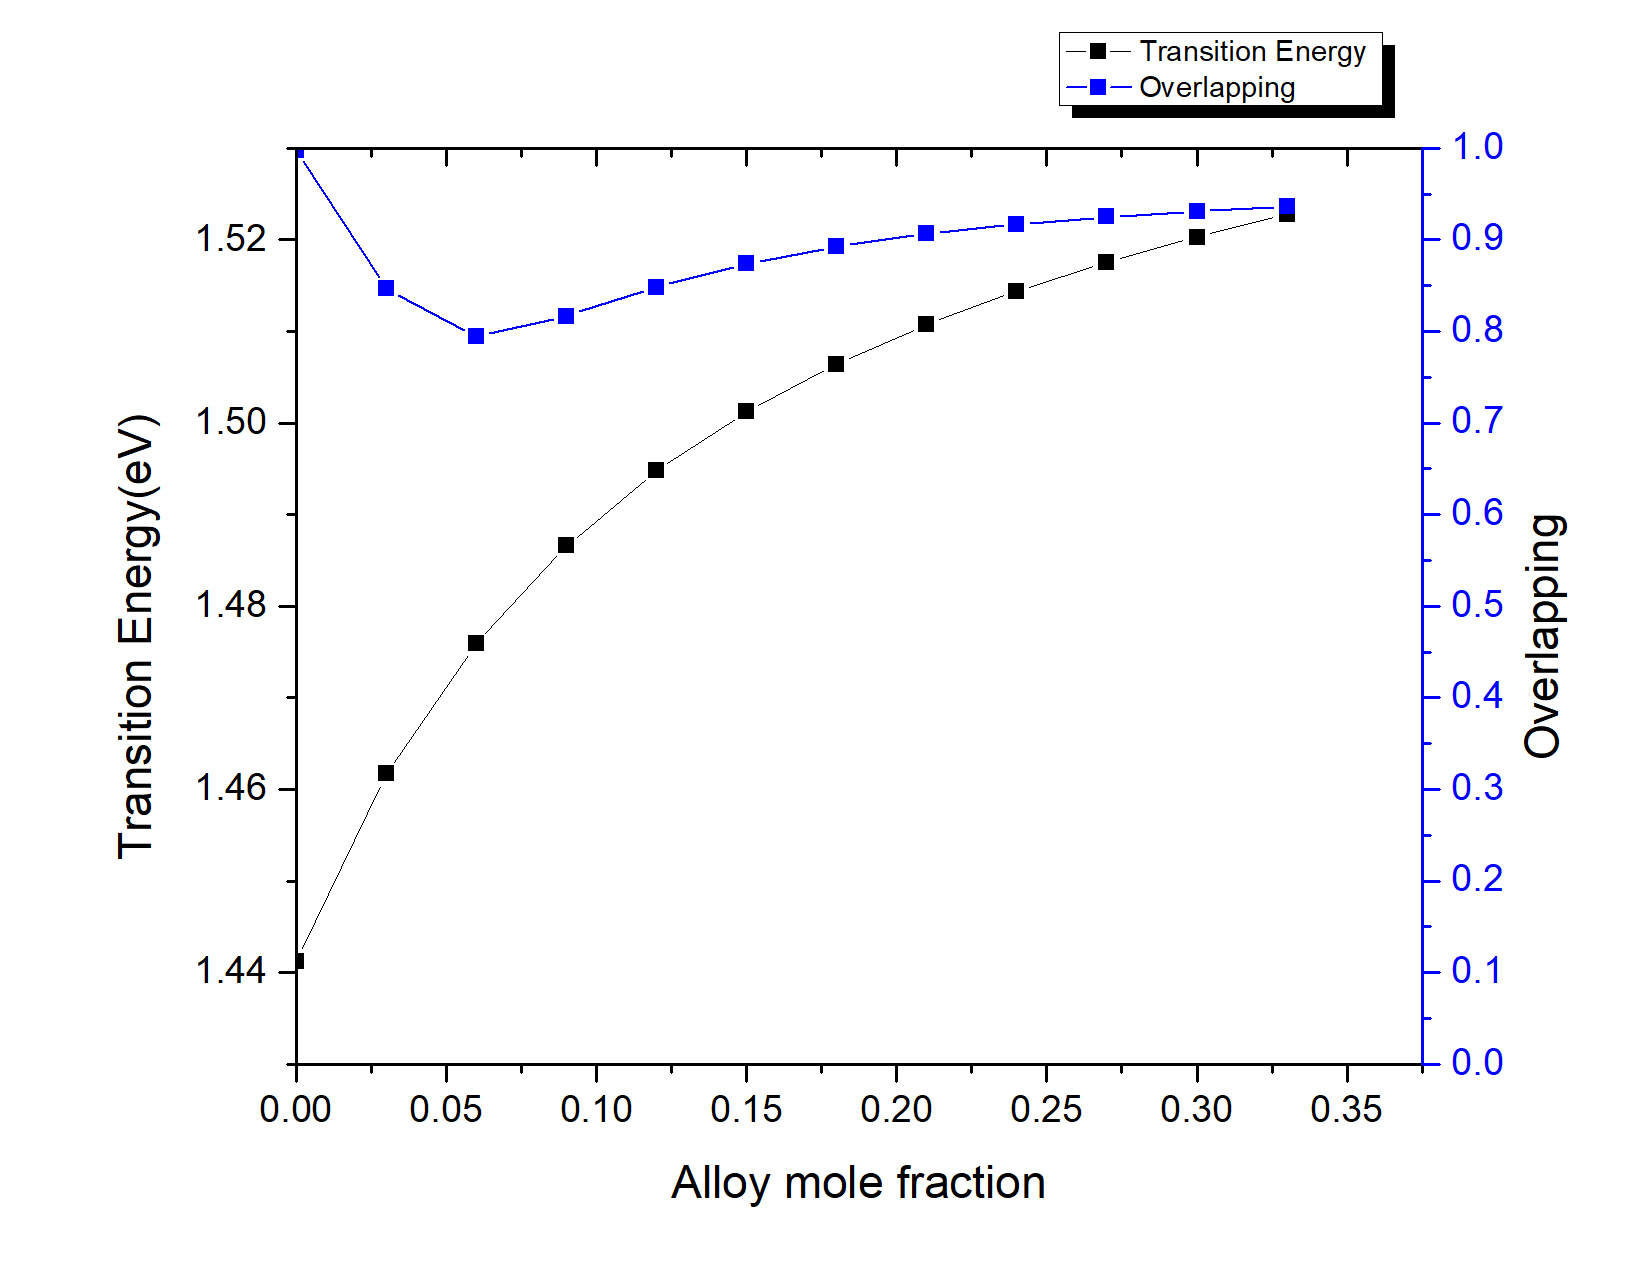
\includegraphics[width=0.8\textwidth]{pictures/RM/AlloySweepMatrixElements}
  \label{AlloySweepMatrixElements}
\end{figure}

\subsection{Oscillator Strength}

According to Thomas-Reiche-Kuhn (TRK) sum rule~\cite{wang1999generalization},
the integrated oscillator strength of an absorber equals the total number of
electrons in the structure. The increased number of photo-induced electrons in
lower-dimensional electronic states manifest in proportional increase in
probability of optical transition. The optical matrix element for the
electron-to-heavy hole transition induced oscillator strength per unit length
can be expressed as:

\begin{equation}
\frac{f_0}{L}=\frac{2{p_{cv}^2}}{{E_g}{m_0}}{|\int{\Psi_0^{(e)}}(x,z){\Psi_0^{(h)}}(x,z)\,{\mathrm{d}x}\,{\mathrm{d}z}\,F_{ex}(r)|}^2,
\label{eq:OscillatorStrength}
\end{equation}
where the squared part is the exciton wave function with $F_{ex}(r)$ being the
envelope part; ${\Psi_0^{(e)}}(x,z)$ and ${\Psi_0^{(h)}}(x,z)$ are the ground
state wave functions for electrons and heavy holes, respectively, in the
absence of their interaction. Esaki et al.~\cite{Chang:1985jz} have
demonstrated that the oscillator strength per unit volume of a GaAs/AlGaAs
quantum wire is $3 \times 10^{-5} {\text{\normalfont\AA}}^{-3}$, nearly an
order of magnitude larger than for bulk GaAs value of $3.5 \times 10^{-6}
{\text{\normalfont\AA}}^{-3}$ as shown in Fig.~\ref{OscillatorStrength}.

\begin{figure}
  \caption[Exciton binding energy (solid) and oscillator strength per unit length (dashed) vs well thicknesses $d_0$ and $d_1$.]{Exciton binding energy (solid) and oscillator strength per unit length (dashed) vs well thicknesses $d_0$ and $d_1$. Figure adapted from reference~\cite{Chang:1985jz}.}
  \centering
  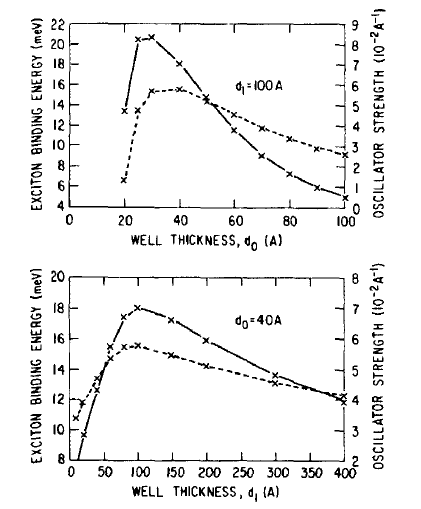
\includegraphics[width=0.6\textwidth]{pictures/RM/OscillatorStrength}
  \label{OscillatorStrength}
\end{figure}

\subsection{Joint Optical Density of States}

Thirdly, the joint optical density of states (JDOS) function is strongly
dependent on dimensionality which comes from the summation over wave numbers k,
from continuous JDOS for 3D to step-like JDOS for 2D, and discrete form for 1D,
as explicitly shown in Eqs.~(\ref{eq:3DDOS}, \ref{eq:2DDOS} and
\ref{eq:1DDOS}). As this function connects electron hole pairs involved in a
transition, it has a reduced effective mass
$\frac{1}{m_r^\ast}=\frac{1}{m_e^\ast}+\frac{1}{m_h^\ast}$ which for 3D is
equivalent to that of electrons, but in 2D and 1D changes substantially due to
separation of heavy, light, and split-off bands in valence band. In fact, the
hole effective mass is reduced to $0.027m_0$ for 1D quantum wire structure, and
to $0.118m_0$ for 2D quantum well, compared with $0.51m_0$ for bulk
GaAs~\cite{Suemune:1988jw} as shown in Fig.~\ref{EffectiveMass}.

\begin{figure}
  \caption[Effective mass value estimated in the wire direction in the lowest valence subband of $GaAs/Al_xGa_{1-x}As$ quantum wire.]{Effective mass value estimated in the wire direction in the lowest valence subband of $GaAs/Al_xGa_{1-x}As$ quantum wire. The solid line is the finite barrier model. The dashed line is the infinite barrier model, where the effective mass value is independent of the well width. The maximum wave vector where the parabolic approximation holds within the accuracy of 1 meV is also shown. Figure adapted from reference~\cite{Suemune:1988jw}.}
  \centering
  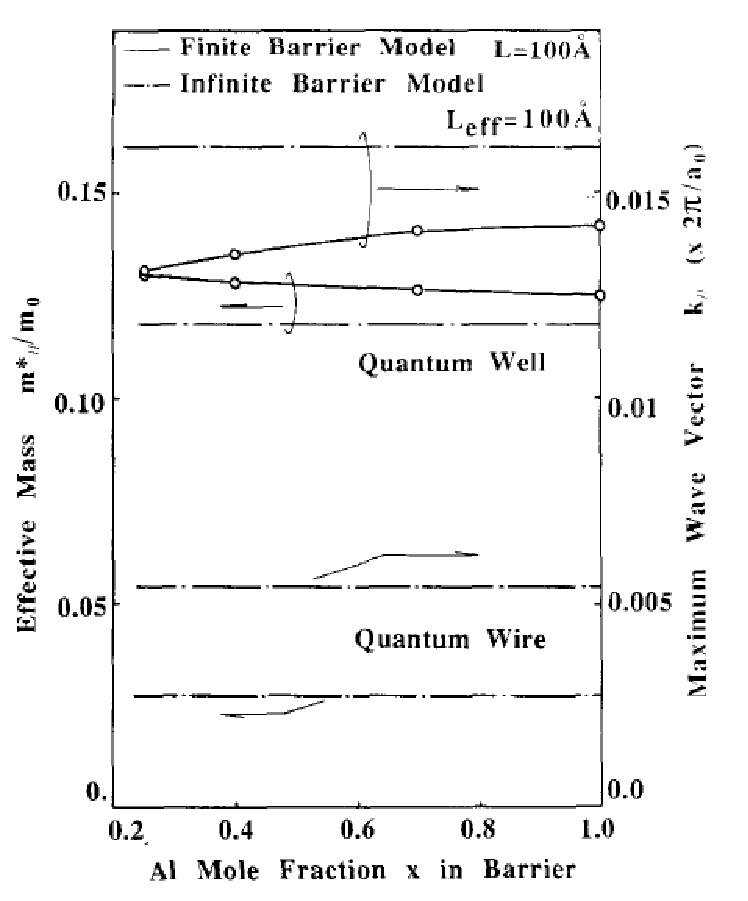
\includegraphics[width=0.8\textwidth]{pictures/RM/EffectiveMass}
  \label{EffectiveMass}
\end{figure}

\begin{equation}
\rho_r^{3D}=\frac{1}{2\pi^2}(\frac{2m_r^\ast}{\hbar^2})^{3/_2}(\hbar\omega-E_g)^{1/_2}
\label{eq:3DDOS}
\end{equation}

\begin{equation}
\rho_r^{2D}=\frac{m_r^\ast}{\pi\hbar^2{L_z}}
\label{eq:2DDOS}
\end{equation}

\begin{equation}
\rho_r^{1D}=\frac{{(m_r^\ast)}^{3/_2}}{\pi\hbar{m_e^\ast}{L_x}{L_y}}\frac{1}{\sqrt{(\hbar\omega-E_g)}}
\label{eq:1DDOS}
\end{equation}

\section[Spacial Overlapping]{Spacial Overlapping of confined light and electronic wavefunctions}

The electronic band structure of hexagonal core-shells is calculated
self-consistently by solving Poisson and Schr{\'o}dinger equations showing
that, as expected, at high doping concentrations of the shell two-dimensional
electron gasses (2DEG) form at the six (6) core-shell heterointerface facets,
with six (6) pillars of one-dimensional electron gas (1DEG) forming at the six
vortices; this is schematically shown in Fig.~\ref{PhotonCharge}(a). The
electronic wave function is calculated and shown in Fig.~\ref{PhotonCharge}(b)
for core of GaAs and shell of AlGaAs, with high doping assumed for the shell,
in two cuts: one along two opposing vortices and one along two opposing facets.
Clearly, 2DEG and 1DEG exist, respectively, at facets and vortices. Calculation
of transition rates with incorporation of dimensionality shows over one order
of magnitude increase for the 2D and over two orders of magnitude for 1D
compared to the same material in 3D. Furthermore, for the stimulated emission
rate calculation, the mode occupancy number $u_\varepsilon$ in
Eq.~\ref{eq:occupationfactor} plays an important role, as expected.

\begin{figure}
  \caption[The schematic plot of GaAs/AlGaAs core-shell nanowire electron charge distribution with band bending, and the FTDT-simulated (optical) electric field intensity distribution.]{(a) The schematic plot of GaAs/AlGaAs core-shell nanowire with electron charge positions. (b) The calculated conduction band energy diagram and the electron density at y cross section (top) and x cross section (bottom) with high doping density. (c) FDTD-simulated (optcial) electric field intensity of a hexagonal nanowire at y cross section (top) and x cross section (bottom). The insets are mode patterns ($TM_{5n}$) in the transverse plane. The black boundaries represent the interface between semiconductor and air.}
  \centering
  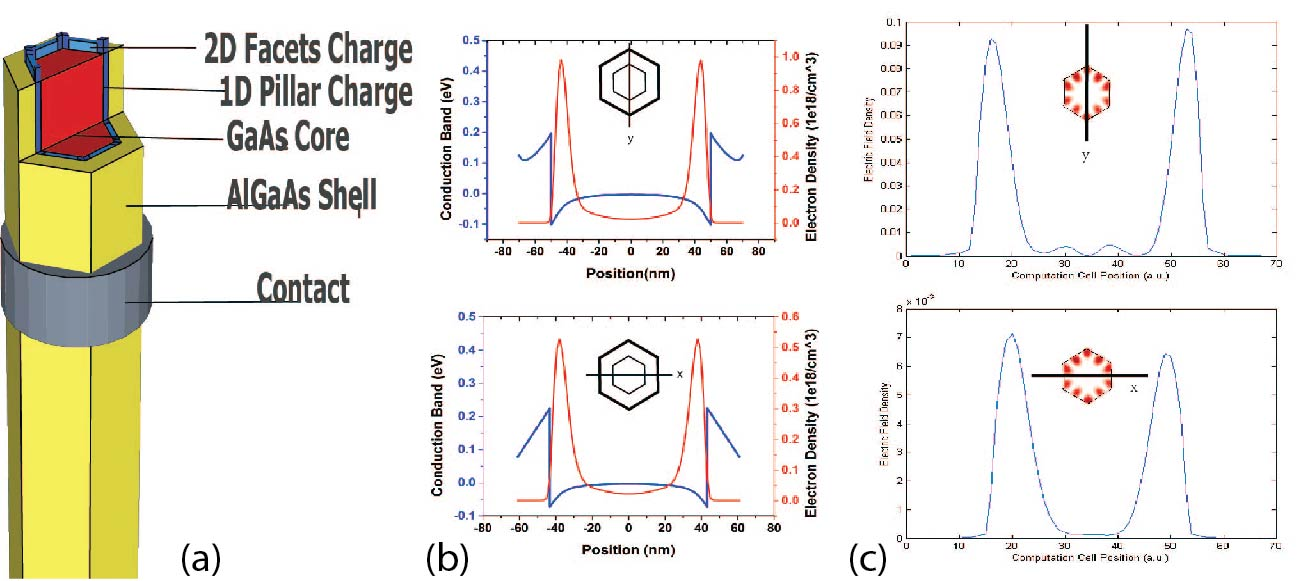
\includegraphics[width=\textwidth]{pictures/ED/Photoncharge}
  \label{PhotonCharge}
\end{figure}

Figure~\ref{PhotonCharge}(C) shows the FDTD-simulated electric field density
of a hexagonal nanowire at y cross section (top) and x cross section (bottom).
The photon energy of this mode shown as the insets of Fig.~\ref{PhotonCharge}
(C) is concentrated primarily along the 6 corners and secondarily along the
facets with little light in the 3D core of GaAs. Hence, we suggest that the
fortuitous spatial overlap of the resonant optical modes on reduced dimensional
electronic wavefunctions plays a significant role in the remarkable
optoelectronic properties of core-shell nanowires. Restated, the superposition
of the photon modes on reduced electronic states that form on the facets and
vortices of the hexagonal CSNWs strongly enhances both upward and downward
transition rates. Thus, the reduced dimensionality transition rate
distinguishes the core-shell nanostructure from the optically equivalent
core-only structure due to its significantly modified rate management. These
nanostructures are not only excellent optical cavities, but despite their large
size also provide the right reduced dimensional electronic structures which
enhance optoelectronic interactions. It should be noted the present analysis
is for direct optical transitions; although it can be extended to incorporate
k-vector changes as in phonon scattering, other important factors such as
many-body interactions need to be included in a more detailed analysis.

\section{Many body effects}

The preceding discussion of dimensional dependent optical transition rates
involving time-dependent perturbation theory and Fermi's Golden Rule considers
each electron in isolation as it interacts with the electromagnetic field. In
this derivation, a single-particle theory has been used to obtain the optical
transition rates and the optical gain spectrum, which will be presented in
Chapter~\ref{LT}. In reality, there is a large density of both electrons and
holes present in the system. The mutual interactions between these particles
are generally referred to as many-body effects~\cite{coldren2012diode}. These
effects included lineshape broadening, which is related to collisions between
particles and/or phonons in the crystal and will also be discussed in
Chapter~\ref{LT}. In addition to this important effect, there are two other
significant consequences of many-body effects: exciton
states~\cite{Suemune:1988jw} and bandgap shrinkage~\cite{Wang:2001to}. Exciton
states exist primarily at low carrier densities and low temperatures, where
bandgap shrinkage becomes noticeable at high carrier densities.

Exciton pair can be formed under conditions of low carrier density and low
temperature, as there is possibility that an electron and hole to orbit each
other for an extended period of time.  Such exciton pairs have a binding energy
associated with them that is equal to the energy required to separate the
electron and hole. As a result, electrons that are elevated from the valence
band to one of these exciton states will absorb radiation at energies equal to
the bandgap substracting the binding energy (the bandgap will appear to be
red-shifted). In addition, the overlap integral (and hence the matrix element)
of these two-particle states can be quite large. As a result, band-to-exciton
transitions tend to dominate the absorption spectrum.  However, exciton states
are limited to states near $k = 0$, and hence band-to-exciton transitions are
clustered at the band edge (or subband edge). The overall effect is the
appearance of very strong absorption peaks near the subband edges in
two-dimensions or one-dimension electronic states, and near the band edge in
bulk case~\cite{coldren2012diode}.

Exciton absorption peaks are clearly visible in quantum wells at room
temperature for a typical GaAs QW. The first two steps in the "staircase"
absorption spectrum predicted from the density of states. However, the exciton
peaks riding on top of the steps, particularly the $n = 1$ peaks, dominate the
absorption spectrum. Each observed exciton peak corresponds to one of the
subband transitions. This phenomenon will become more prominent in
one-dimensional case with discrete joint optical density of states.

The second many-body effect occurs at high carrier densities, where the charges
actually screen out the atomic attractive forces. With a weaker effective
atomic potential, the single-atom electron wavefunctions of interest become
less localized and the nearest-neighbor electron overlap becomes higher. The
large overlap increases the width of the energy bands ($\delta{E}$ is larger),
reducing the gap between bands. Although this description is only qualitative,
it does reveal that the bandgap should shrink with increasing carrier
density~\cite{coldren2012diode}. And this bandgap shrinkage is inversely
related to the average spacing between carriers, which means the closer the
carriers are, the more their own Coulomb potentials screen out the atomic
potential.  The net effect of bandgap shrinkage is that as carrier density
increases, the entire gain spectrum red-shifts by a noticeable amount.  In
principle, the shift is accompanied by a slight distortion (i.e, reshaping and
enhancement) of the spectrum.
